\section{Introduction}\label{sec:intro}
%\begin{itemize}
%	\item Generally introduce dialog acts
%	\item Need for automated tagging
%	\item Current SotA
%	\item Introduce distributional representations
%	\item Present hypotheses
%	\item ...
%	\item Set up rest of report
%\end{itemize}
Discourse structure analysis is fundamental in the search for understanding spontaneous dialogs, and developing human-computer dialog systems. An essential part of discourse structure analysis is the identification of Dialog Acts classes (i.e. \emph{questions}, \emph{self-talks}, \emph{statements}, \emph{backchannels}). As defined by Austin \lau{add citation}, Dialog Acts present linguistic abstractions of the illocutionary force of speech acts and model the communicative intention of an utterance in a conversation. There exists several tasks that have Dialog Acts as an input for their computations, examples of these include: speech recognition, speech synthesizer, summarization, and of course, human-machine dialog system construction. As a result, correctly identifying Dialog Act tags is a key point that can lead to improvement in performance of these assignments.
Several approaches had been taken in order to classify Dialog Acts; most of them rely on supervised trained models, and use hand crafted features extracted from the utterance set. \lau{is this true?} We briefly present some of the most relevant researches in the next section.
For the purposes of this work, we take an unsupervised approach to classification. We start by building a distributional semantic model in order to learn vector representations for utterances and then use these vector features as inputs for different machine learning classification models. Neural networks for semantics has gained relevant importance in the past years, since the publication of the first neural networks word embedding models. One of the main reasons for this to happen, is the fact that the resulting vector representations are able to effectively capture the meaning of words given their context. Figure~\ref{fig:w2v_example} shows a typical example of this characteristic.

\begin{figure}
\centering
\begin{minipage}{.4\textwidth}
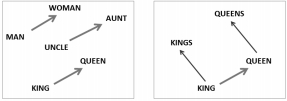
\includegraphics[width=1\textwidth]{img/w2v_example}
\caption{Word2vec semantic relations.}
\label{fig:w2v_example}
\end{minipage}
\end{figure}

In these models, word embeddings are learned by predicting words within a context (depending on the neural network model -i.e. CBOW or Skip-gram, it could be that the network tries to predict a word given a context, or the context given a word), due to the co-occurrence of words in texts, given the use of a language, these models are capable of successfully coming up with mathematical representations of words. This idea of word co-occurrences is not longer valid when we take sentences as units; a sentence can have -potentially- any other valid sentence before and after. Instead, a neural network for learning representations for sentences has been proposed, in which the sentence structures are learned from the words that are included in it. \lau{add cite} In this case, word embeddings and sentence embeddings are trained simultaneously, as a sentence vector, shared across the words within the phrase, is maintained and updated in parallel to the word vectors.  This unsupervised model makes it possible to map sentences (utterances) of any length to vectors of fixed length. Moreover, an interesting characteristic of this model is that multiple corpora can be used as input for training, allowing us to create huge training sets, based on several dialog corpora from different domains and characteristics.

We experiment with different machine learning models in order to automatically classify Dialog Acts. We aim at compare our results with other researches, in terms of feature engineering, and study the usefulness of utterance embeddings in a Dialog Act classification task, while it is beyond the goals of this report to investigate the optimal settings for these classifiers. Experiments were run using the following classification techniques \lau{add classifiers. KNN, NB, MLP, SVM. Comment on default values. This is more methodology}.

The outline of this report is set as follows: in Section 2, we present relevant approaches that aim at classifying Dialog Acts, we briefly describe their main characteristics and results. In Section 3, we specify the datasets used in our experiments and we detail the hows and whys of our classification pipeline. An exhaustive analysis of the results of the experiments is presented in Section 4. And finally, Section 5 includes the conclusions drawn from this work.